%%%%%%%%%%%%%%%%%%%%%%%%%%%%%%%%%%%%%%%%%%%%%%%%%%%%%%%%%%%%%%%%%%%%%%%%%%%%%%%%%%%%%%%%%%%%%%%%%%%%%%%%%%%%%%%%%%%%%%
\chapter{Results for separable $p$}%%%%%%%%%%%%%%%%%%%%%%%%%%%%%%%%%%%%%%%%%%%%%%%%%%%%%%%%%%%%%%%%%%%%%%%%%%%%%%%%%%%
%%%%%%%%%%%%%%%%%%%%%%%%%%%%%%%%%%%%%%%%%%%%%%%%%%%%%%%%%%%%%%%%%%%%%%%%%%%%%%%%%%%%%%%%%%%%%%%%%%%%%%%%%%%%%%%%%%%%%%
We will start by showing correctness of the methods with a convergence plot in section \ref{sec:sconv}, then see if we can find any correlation between $n$ and $\rho$ in section \ref{sec:rrest}.
We compare computation times for the different methods to each other and their predicted computational complexity in section \ref{sec:stimem} and \ref{sec:stimek}.
We will end by seeing how $\gamma$ and $\epsilon$ scales with $\delta$ in section \ref{sec:div}.
%%%%%%%%%%%%%%%%%%%%%%%%%%%%%%%%%%%%%%%%%%%%%%%%%%%%%%%%%%%%%%%%%%%%%%%%%%%%%%%%%%%%%%%%%%%%%%%%%%%%%%%%%%%%%%%%%%%%%%
\section{Convergence} \label{sec:sconv}
%%%%%%%%%%%%%%%%%%%%%%%%%%%%%%%%%%%%%%%%%%%%%%%%%%%%%%%%%%%%%%%%%%%%%%%%%%%%%%%%%%%%%%%%%%%%%%%%%%%%%%%%%%%%%%%%%%%%%%



\begin{figure}[H]
        \centering
        \begin{subfigure}[b]{0.45\textwidth}
                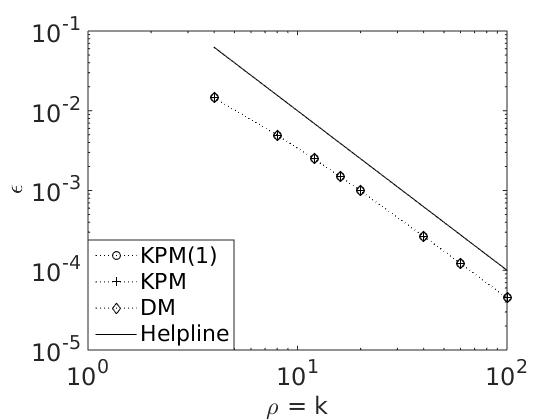
\includegraphics[width=\textwidth]{fig/s1conv1}
                \caption{function \texttt{P1}}
                \label{fig:conv1}
        \end{subfigure}%
~
        \begin{subfigure}[b]{0.45\textwidth}
                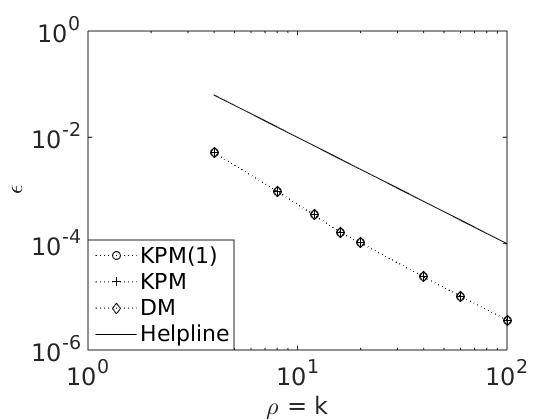
\includegraphics[width=\textwidth]{fig/s2conv2}
                \caption{function \texttt{P2}}
                \label{fig:conv2}
        \end{subfigure}
        \caption{A convergence plot for several method with $\rho = k$. The helpline shows quadratic convergence.}\label{fig:conv}
\end{figure}
As can be seen from figure \ref{fig:conv}, all method converges quadratically and overlap perfectly, this shows us that all method preforms as expected regarding convergence.
%%%%%%%%%%%%%%%%%%%%%%%%%%%%%%%%%%%%%%%%%%%%%%%%%%%%%%%%%%%%%%%%%%%%%%%%%%%%%%%%%%%%%%%%%%%%%%%%%%%%%%%%%%%%%%%%%%%%%%
\section{Choosing restart variable }
%%%%%%%%%%%%%%%%%%%%%%%%%%%%%%%%%%%%%%%%%%%%%%%%%%%%%%%%%%%%%%%%%%%%%%%%%%%%%%%%%%%%%%%%%%%%%%%%%%%%%%%%%%%%%%%%%%%%%%
\begin{figure}[H]
        \centering
        \begin{subfigure}[b]{0.45\textwidth}
                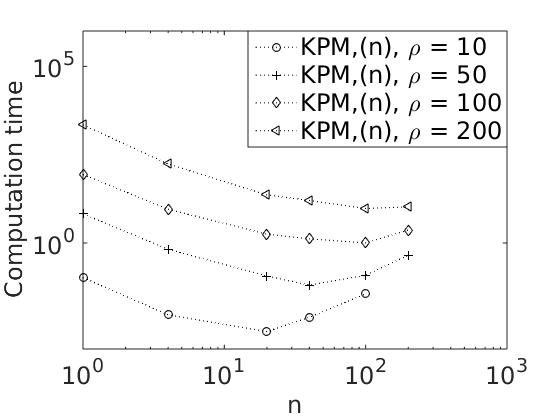
\includegraphics[width=\textwidth]{fig/s9rest1}
                \caption{function \texttt{P1}}
                \label{fig:rest1}
        \end{subfigure}
~
        \begin{subfigure}[b]{0.45\textwidth}
                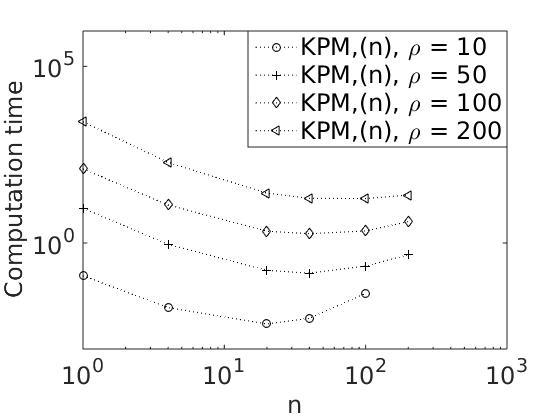
\includegraphics[width=\textwidth]{fig/s10rest2}
                \caption{function \texttt{P2}}
                \label{fig:rest2}
        \end{subfigure}
        \caption{Computation times plotted against restart variable $n$.}\label{fig:rest}
\end{figure}
As we can see from figure \ref{fig:rest}, the optimal restart variable changes as a function of $\rho$ so that larger $\rho$ needs larger $n$ to preform optimally. One point is missing from KPM$(n)$, $\rho = 10$ this is because the last point plotted is the same as KPM. $n = 40$ seams like a good restart variable for these $\rho$.
%%%%%%%%%%%%%%%%%%%%%%%%%%%%%%%%%%%%%%%%%%%%%%%%%%%%%%%%%%%%%%%%%%%%%%%%%%%%%%%%%%%%%%%%%%%%%%%%%%%%%%%%%%%%%%%%%%%%%%
\section{Comparing $\gamma$ and $n$} \label{sec:rrest}
%%%%%%%%%%%%%%%%%%%%%%%%%%%%%%%%%%%%%%%%%%%%%%%%%%%%%%%%%%%%%%%%%%%%%%%%%%%%%%%%%%%%%%%%%%%%%%%%%%%%%%%%%%%%%%%%%%%%%%
\begin{figure}[H]
        \centering
        \begin{subfigure}[b]{0.45\textwidth}
                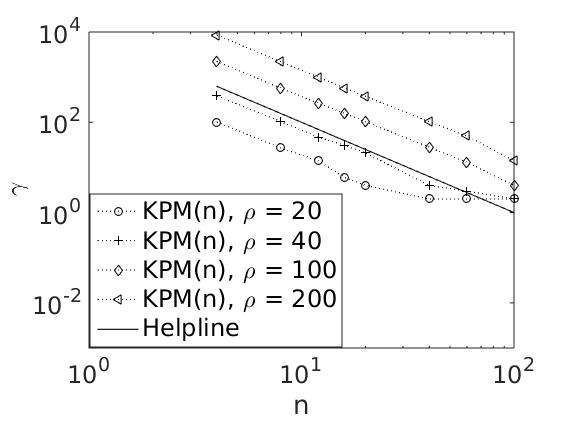
\includegraphics[width=\textwidth]{fig/s3antvsm1}
                \caption{function \texttt{P1}}
                \label{fig:ant1}
        \end{subfigure}%
~
        \begin{subfigure}[b]{0.45\textwidth}
                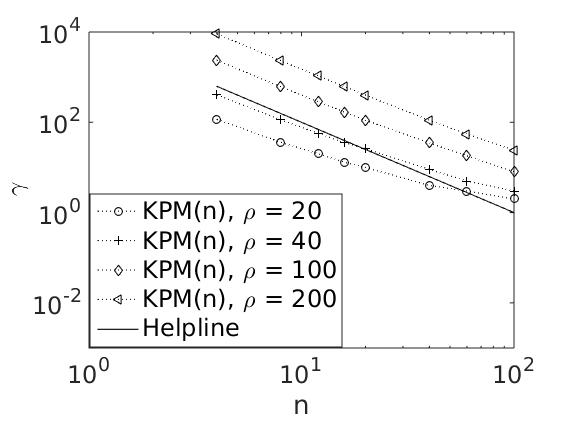
\includegraphics[width=\textwidth]{fig/s4antvsm2}
                \caption{function \texttt{P2}}
                \label{fig:ant2}
        \end{subfigure}
        \caption{The number of restarts, $\gamma$ needed for KPM$(n)$ to converge as a function of $n$. The helpline decreases with $n^2$.}\label{fig:ant}
\end{figure}
As we can see from figure \ref{fig:ant}, $\gamma$ decreases quadratically when $n$ is small, but decreases less when $n$ is larger. If we put this together with the estimated complexity found in section \ref{sec:rrest}, we get that KPM$(n)$ has at most the same estimated complexity as KPM. Notice that the Helpline follows $m^2/n^2$, as suggested in section \ref{sec:cc}.
%%%%%%%%%%%%%%%%%%%%%%%%%%%%%%%%%%%%%%%%%%%%%%%%%%%%%%%%%%%%%%%%%%%%%%%%%%%%%%%%%%%%%%%%%%%%%%%%%%%%%%%%%%%%%%%%%%%%%%
\section{Computation time for $m$} \label{sec:stimem}
%%%%%%%%%%%%%%%%%%%%%%%%%%%%%%%%%%%%%%%%%%%%%%%%%%%%%%%%%%%%%%%%%%%%%%%%%%%%%%%%%%%%%%%%%%%%%%%%%%%%%%%%%%%%%%%%%%%%%%
\begin{figure}[H]
        \centering
        \begin{subfigure}[b]{0.45\textwidth}
                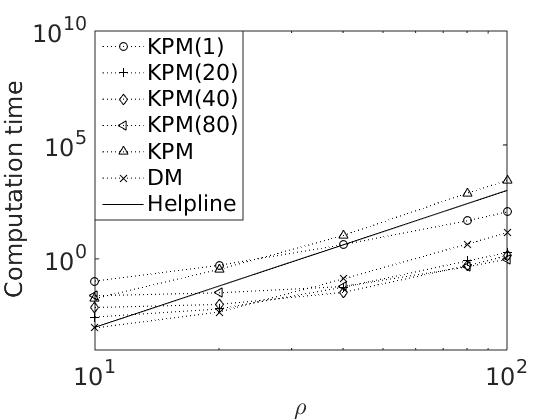
\includegraphics[width=\textwidth]{fig/n5timevsm1}
                \caption{function \texttt{P1}}
                \label{fig:timem1}
        \end{subfigure}%
        ~
        \begin{subfigure}[b]{0.45\textwidth}
                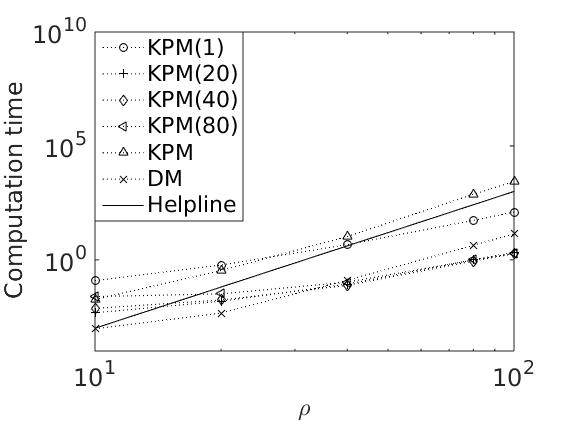
\includegraphics[width=\textwidth]{fig/n6timevsm2}
                \caption{function \texttt{P2}}
                \label{fig:timem2}
        \end{subfigure}
        \caption{A plot of computation time as a function of $\rho$, the helpline increases with $\rho^6 = m^3$.}\label{fig:timem}
\end{figure}
As we can see from figure \ref{fig:timem}, the computation time for KPM increases as expected, while DM and KPM$(n)$ increases slower, perhaps due to MATLAB's efficient inversion algorithm and less memory demand. 
Even more interesting is it that KPM$(n)$ is both asymptotically better, and faster than DM for large $\rho$, so clearly KPM$(n)$ is better in some cases.
%%%%%%%%%%%%%%%%%%%%%%%%%%%%%%%%%%%%%%%%%%%%%%%%%%%%%%%%%%%%%%%%%%%%%%%%%%%%%%%%%%%%%%%%%%%%%%%%%%%%%%%%%%%%%%%%%%%%%%
\section{Computation time for $k$} \label{sec:stimek}
%%%%%%%%%%%%%%%%%%%%%%%%%%%%%%%%%%%%%%%%%%%%%%%%%%%%%%%%%%%%%%%%%%%%%%%%%%%%%%%%%%%%%%%%%%%%%%%%%%%%%%%%%%%%%%%%%%%%%%
\begin{figure}[H]
        \centering
        \begin{subfigure}[b]{0.45\textwidth}
                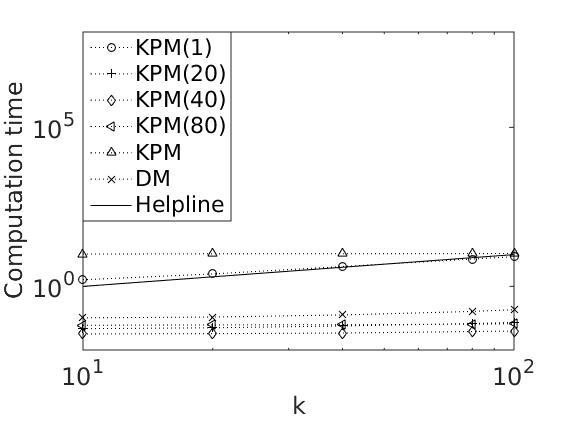
\includegraphics[width=\textwidth]{fig/n7timevsk1}
                \caption{function \texttt{P1}}
                \label{fig:timek1}
        \end{subfigure}%
~
        \begin{subfigure}[b]{0.45\textwidth}
                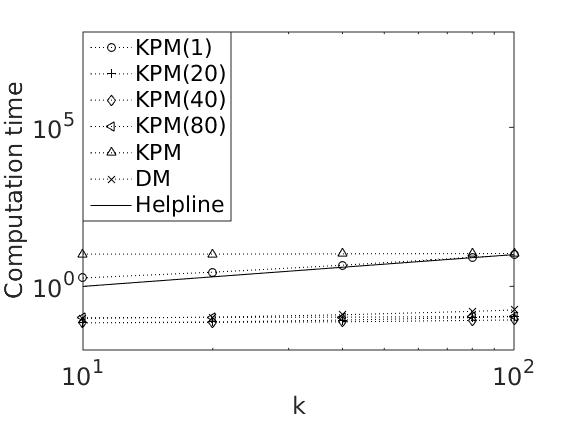
\includegraphics[width=\textwidth]{fig/n8timevsk2}
                \caption{function \texttt{P2}}
                \label{fig:timek2}
        \end{subfigure}
        \caption{A plot of computation time as a function of $k$, the helpline increases with $k$.}\label{fig:timek}
\end{figure}
As we can see from figure \ref{fig:timek}, the computation time for almost all tested methods are constant. The reason is that the time needed for initialising is much greater than the time it takes to integrate. 
The exception is KPM$(1)$, which increases close to linear because relatively more work is done while integrating, due to several restarts.
We also see that KPM$(n)$ is faster than DM for some $n$, KPM is again very slow.
%%%%%%%%%%%%%%%%%%%%%%%%%%%%%%%%%%%%%%%%%%%%%%%%%%%%%%%%%%%%%%%%%%%%%%%%%%%%%%%%%%%%%%%%%%%%%%%%%%%%%%%%%%%%%%%%%%%%%%
\section{Comparing $\delta$ with $\gamma$ and $\epsilon$} \label{sec:div}
%%%%%%%%%%%%%%%%%%%%%%%%%%%%%%%%%%%%%%%%%%%%%%%%%%%%%%%%%%%%%%%%%%%%%%%%%%%%%%%%%%%%%%%%%%%%%%%%%%%%%%%%%%%%%%%%%%%%%%
\begin{figure}[H]
        \centering
        \begin{subfigure}[b]{0.45\textwidth}
                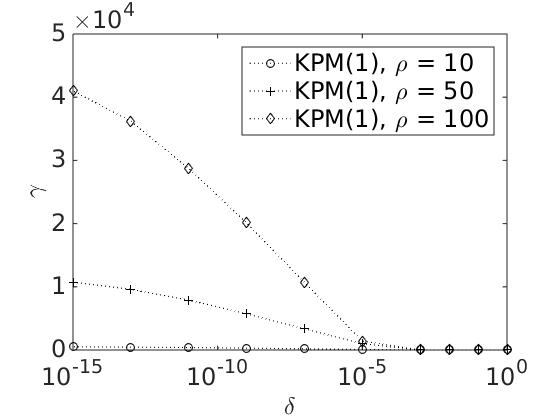
\includegraphics[width=\textwidth]{fig/s13antvstol1m}
                \caption{function \texttt{P1}}
                \label{fig:errant1}
        \end{subfigure}
~
        \begin{subfigure}[b]{0.45\textwidth}
                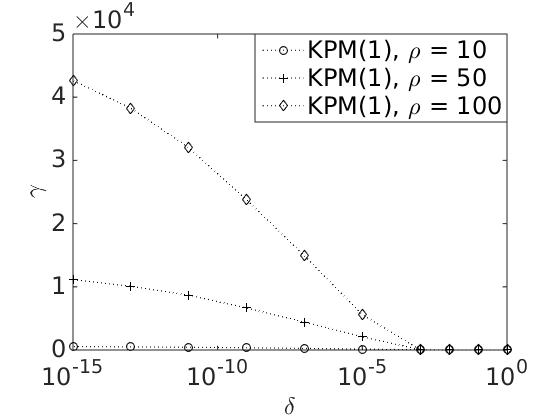
\includegraphics[width=\textwidth]{fig/s14antvstol2m}
                \caption{ function \texttt{P2}}
                \label{fig:errant2}
        \end{subfigure}
        
        \begin{subfigure}[b]{0.45\textwidth}
                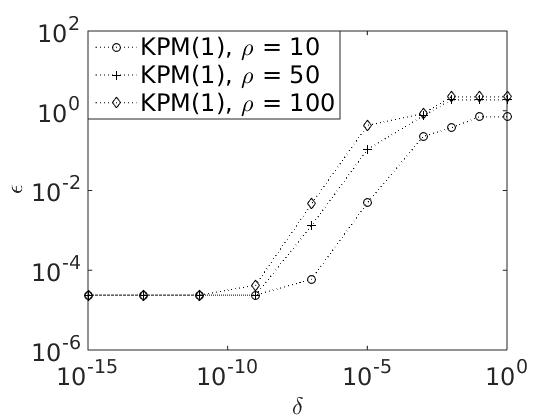
\includegraphics[width=\textwidth]{fig/s15errvstol1m}
                \caption{function \texttt{P1}}
                \label{fig:errtol1}
        \end{subfigure}
~
        \begin{subfigure}[b]{0.45\textwidth}
                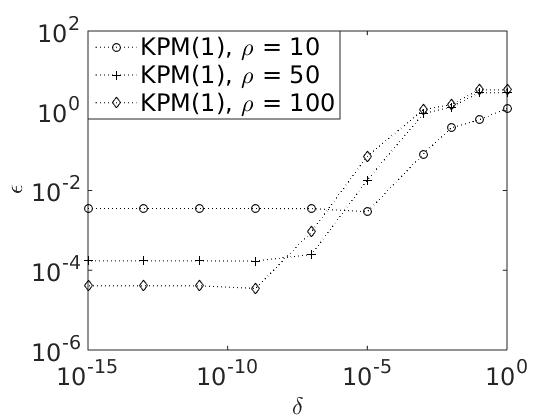
\includegraphics[width=\textwidth]{fig/s16errvstol2m}
                \caption{ function \texttt{P2}}
                \label{fig:errtol2}
        \end{subfigure}
        
        \caption{A plot of $\epsilon$ and $\gamma$ as a function of $\delta$, with different $\rho$.} \label{fig:errant}
\end{figure}
Figure \ref{fig:errant} and \ref{fig:errtolk} shows how $\gamma$ and $\epsilon$ scales with $\delta$. Figure \ref{fig:errtol1} has reached to threshold precision with $k = 40$. Both figures shows a loglinear dependence between $\gamma$ and $\delta$. The figures also shows the importance of choosing an appropriate $\delta$. A lot of time can be saved by choosing $\delta$ larger, but precision is lost if $\delta$ is to large.
\begin{figure}[H]
        \centering
        \begin{subfigure}[b]{0.45\textwidth}
                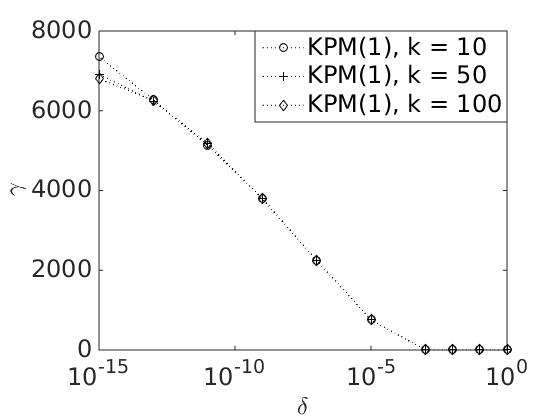
\includegraphics[width=\textwidth]{fig/s20antvstol1k}
                \caption{function \texttt{P1}}
                \label{fig:anttol1k}
        \end{subfigure}
~
        \begin{subfigure}[b]{0.45\textwidth}
                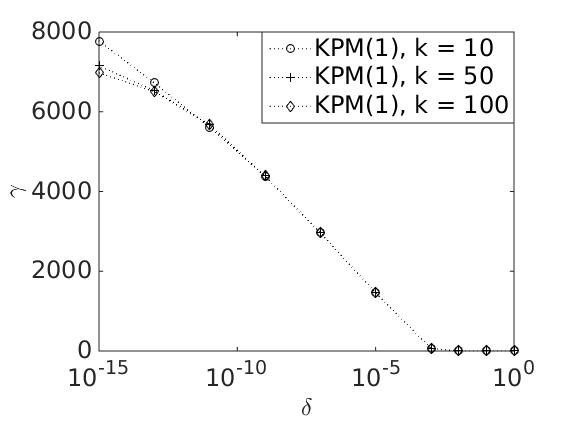
\includegraphics[width=\textwidth]{fig/s21antvstol2k}
                \caption{ function \texttt{P2}}
                \label{fig:anttol2k}
        \end{subfigure}
                \begin{subfigure}[b]{0.45\textwidth}
                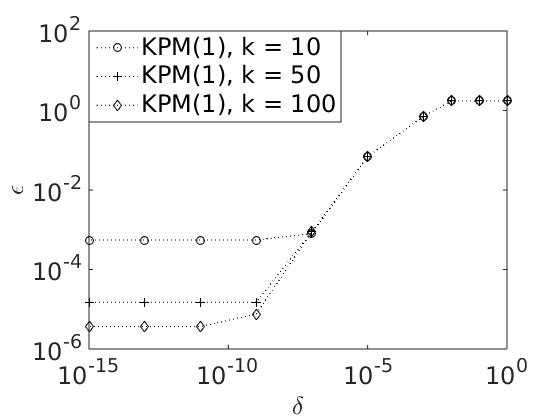
\includegraphics[width=\textwidth]{fig/s22errvstol1k}
                \caption{function \texttt{P1}}
                \label{fig:errtol1k}
        \end{subfigure}
~
        \begin{subfigure}[b]{0.45\textwidth}
                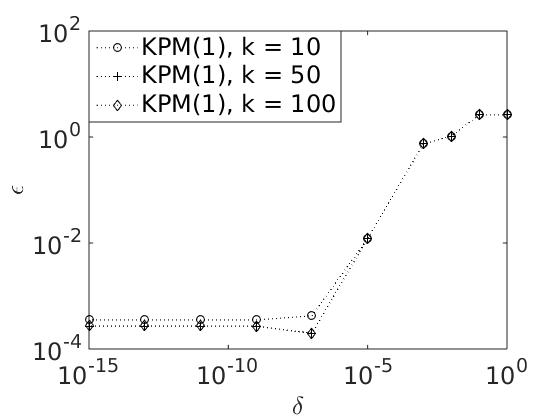
\includegraphics[width=\textwidth]{fig/s23errvstol2k}
                \caption{ function \texttt{P2}}
                \label{fig:errtol2k}
        \end{subfigure}
        \caption{A plot of $\epsilon$ and $\gamma$ as a function of $\delta$, with different $k$.} \label{fig:errtolk}
\end{figure}

\newpage